\section{The Sioux Falls Scenario}
\label{sec:sioux}

The City of Sioux Falls in South Dakota (\cref{fig:original_map}) has been a classic test case in transport
research for more than four decades, being first mentioned in this context in
\citet{Morlok1973}. While none of the numerous implementations of the network are intended to be accurate
and realistic with respect to the actual City of Sioux Falls, they are merely aiming
towards providing downscaled, computationally tractable test cases for transport
planning and simulation problems.

In \citet{Chakirov2014}, the scenario (``Sioux-14'', \cref{fig:sioux14}) has been
adapted to the MATSim framework. A sparse street network, which is computationally
easy to handle by the simulation, was introduced. It consists of 27 nodes and 76 links,
representing the main arterial roads of the city, split further down into
282 nodes and 334 links in order to arrive at partial link sizes of less than $500m$.
This is necessary because MATSim agents start their travels at the start node
of a link and thus a high resolution is needed to avoid unrealistic clustering.

\begin{figure}
    \centering
    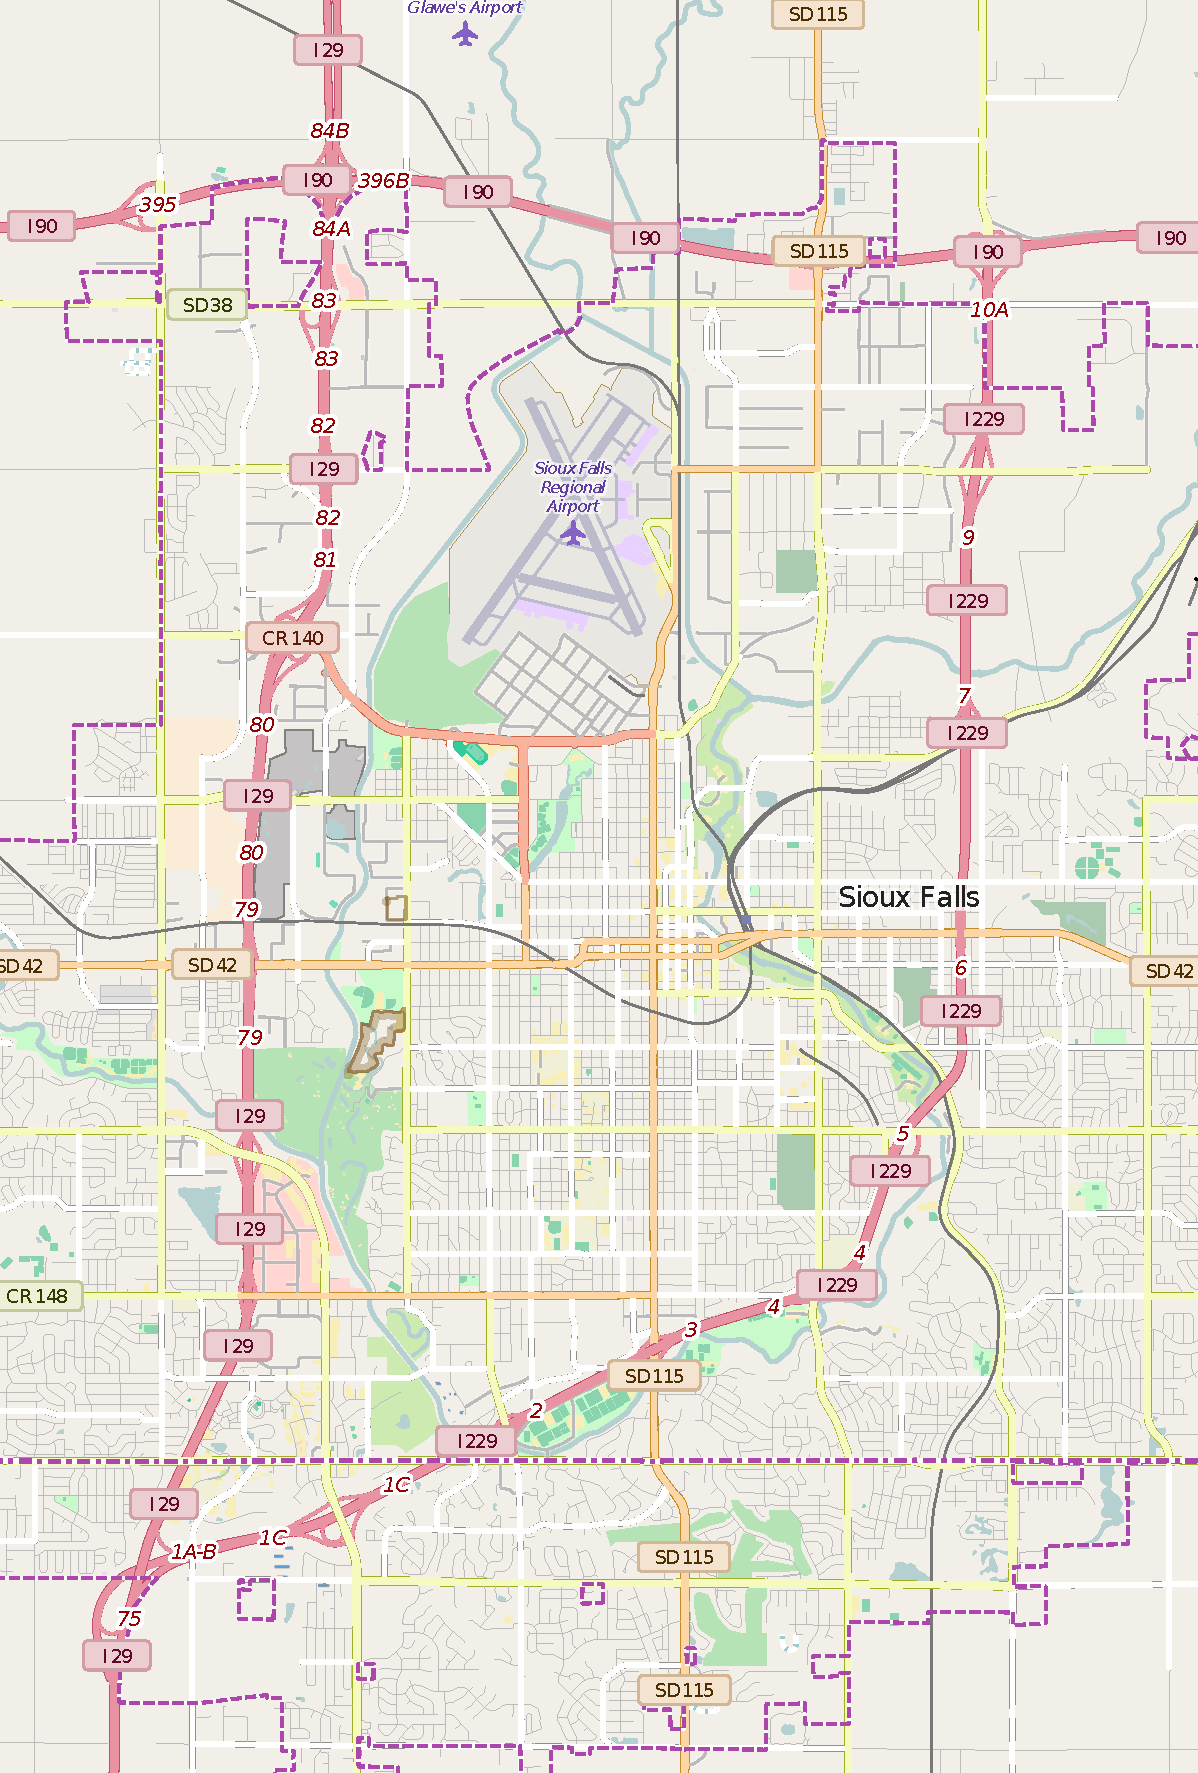
\includegraphics[width=0.8\textwidth]{figures/original_map.pdf}
    \caption{Map of Sioux Falls from OpenStreetMap. Longitude from $-96.8105°$ to $-96.6653°$ and latitude from $43.4729°$ to $43.6286°$.}
    \label{fig:original_map}
\end{figure}

\begin{figure}
    \centering
    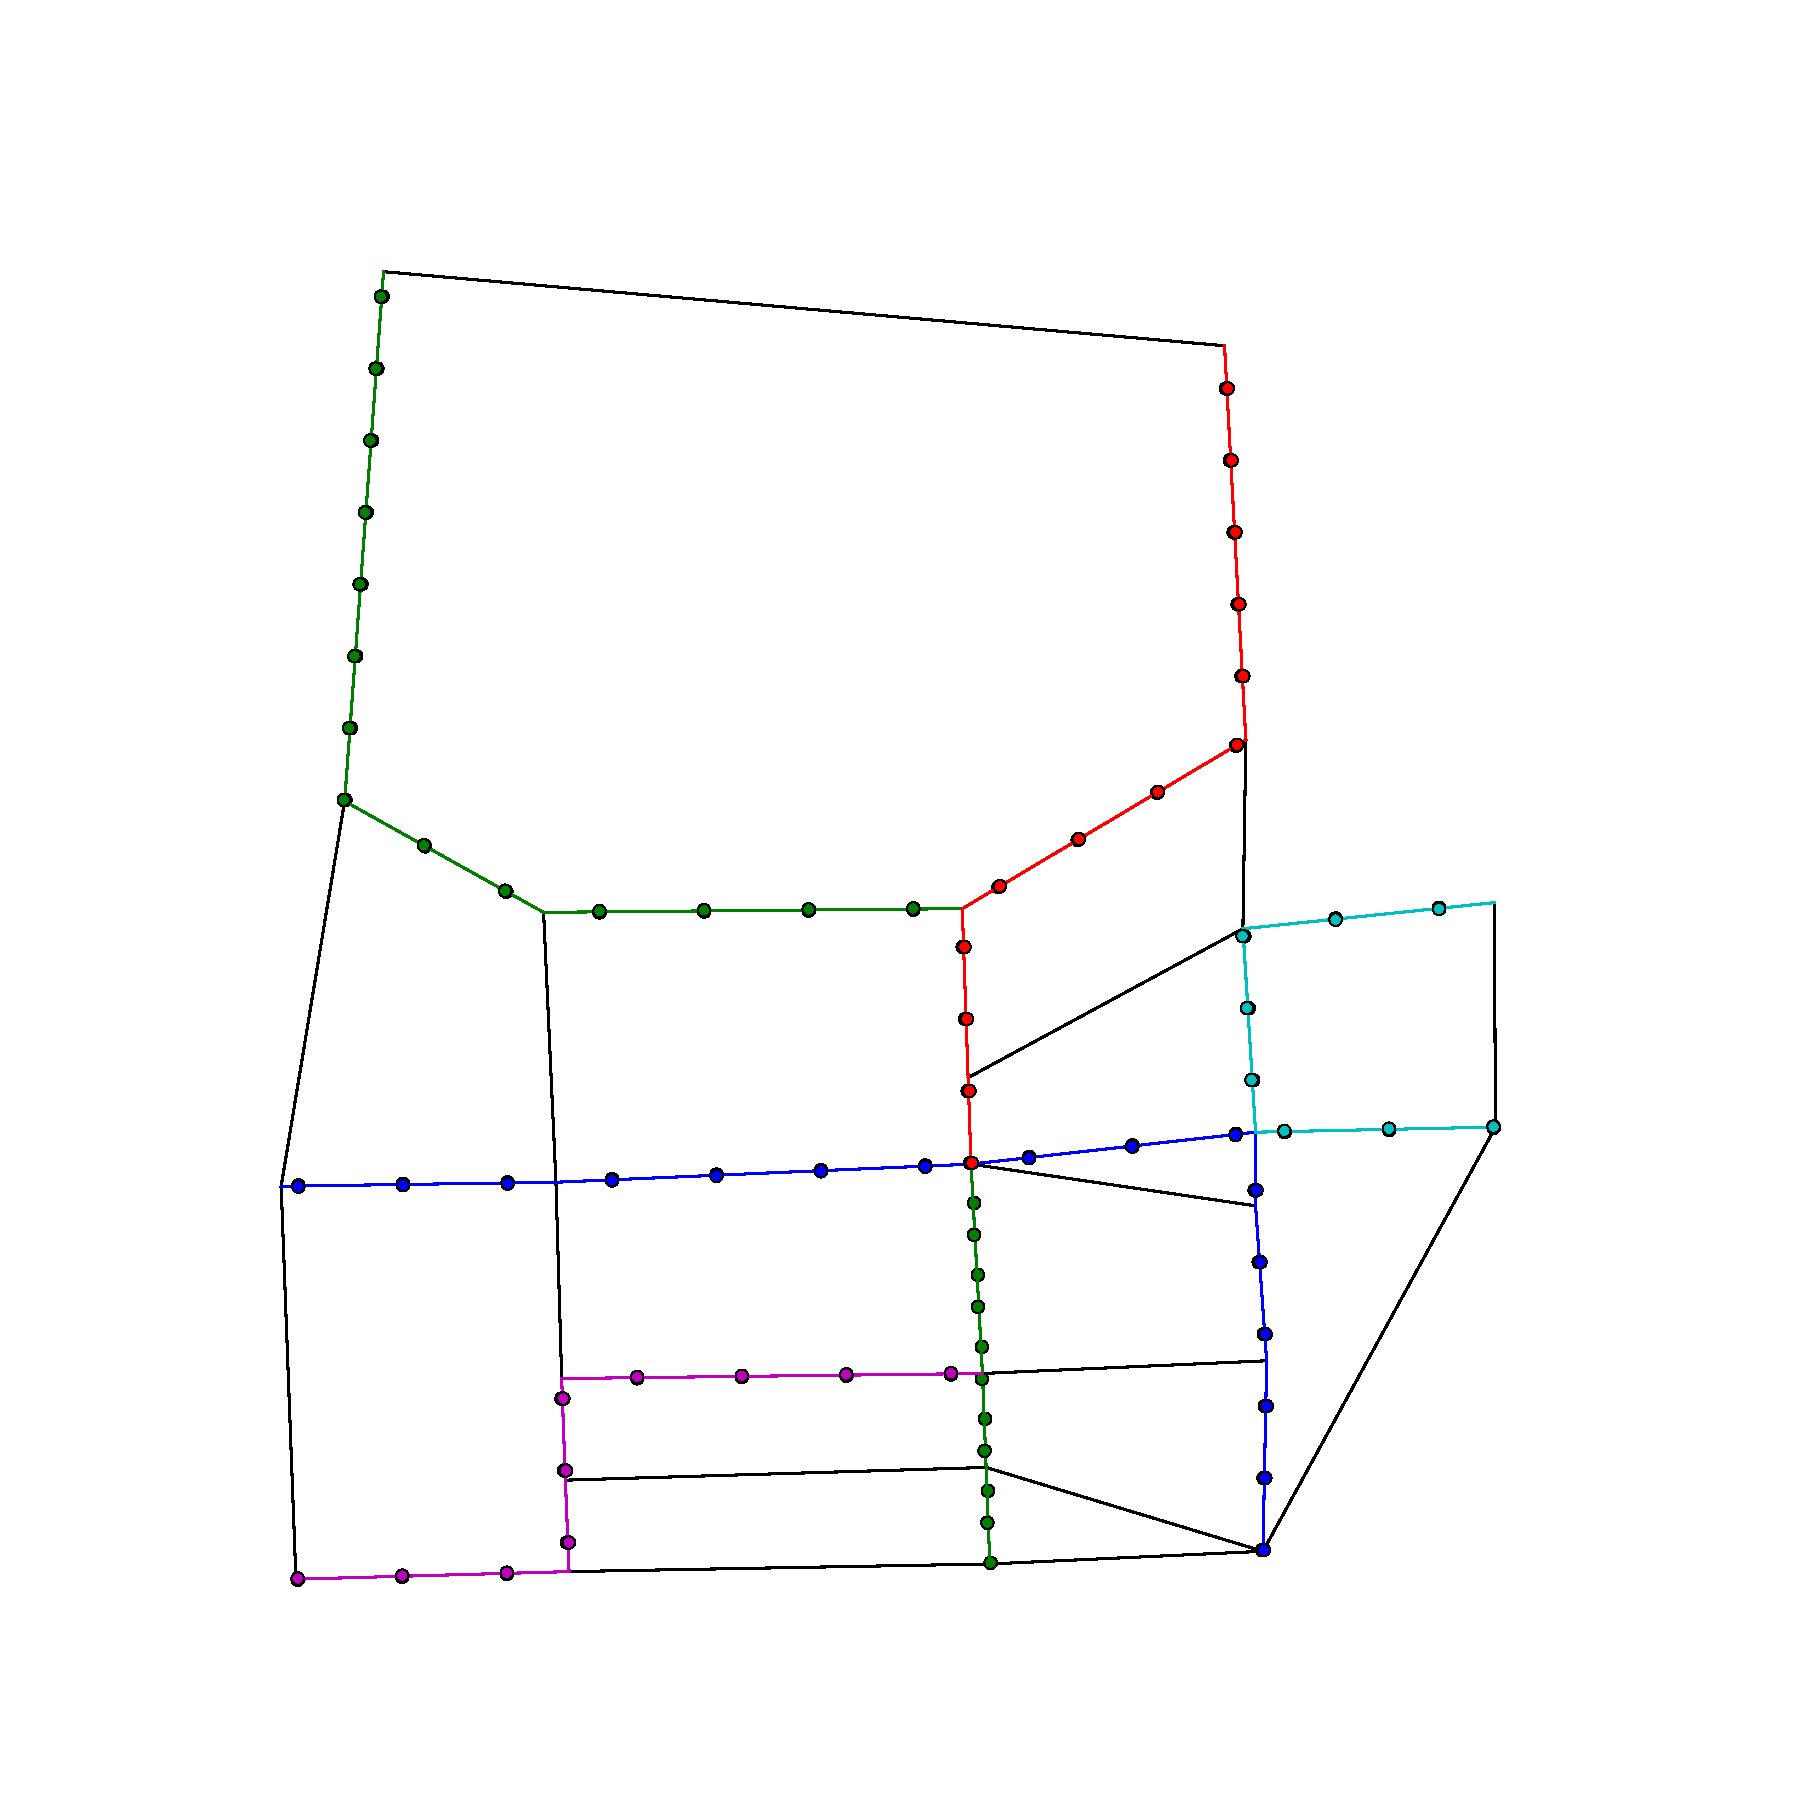
\includegraphics[width=0.6\textwidth]{figures/sioux14_pt.pdf}
    \caption{Sioux-14 road and public transport network}
    \label{fig:sioux14}
\end{figure}

On the supply side, there is furthermore a public transport network, which
consists of 5 lines with bus stops along the arterial roads in a distance of $600m$.
The stops are placed at a distance of $5m$ perpendicular to the road and departures
from the lines' respective start links take place every 5 minutes.

Much of effort has been put into the modeling of the demand side, covering the
realistic generation of home locations, workplaces, secondary activity locations,
as well as the distribution of socio-economic factors such as age, car ownership
and gender across a synthetic population, as it is needed for the agent-based
simulation.

In this regard, the scenario provides a lightweight example of a complete MATSim
simulation, where it is easy to test different parameters and extensions to the
framework on a near-realistic baseline scenario. However, while working with the
original Sioux-14 network during the course of this thesis, it became evident that
the simplified structure of the underlying traffic network does not provide enough
resolution for the simulation of autonomous vehicles.

The main reason is that agents, who choose to take a car in the Sioux-14 network,
probably living in the middle of the rectangular regions of the network would be
teleported to the nearest link to start their travels. This would also be true
for autonomous vehicles, which is not a realistic assumption in both cases, especially
when comparing it with public transport, where agents in MATSim are explicitly
penalized for covering the distance between home and bus stop by foot.
Furthermore, the effect of people being more inclined to opt for an autonomous taxi
when living far from public transport can only be convincingly simulated on a
finer network.

The following sections will describe how, starting from the initial Sioux-14
scenario, a new more fine-grained versatile test scenario for MATSim has been
developed, which in turn has been used as the basis of the following investigations in this
thesis.

The new Sioux-16 network, which has been developed in this thesis, is based on the
demand model of Sioux-14, which means that all locations for homes, workplaces and
secondary activities are kept equal, while it differs on the supply side, aiming
to resemble the original scenario as closely as possible. The following sections
will describe, how the Sioux Falls network from OpenStreetMap (with the state
as of 18 Apr 2016) has been converted and adjusted to be compatible with MATSim
and closely match the prior version of the test scenario. Furthermore, it will
be explained, how the public transport network has been adapted to the fine-grained
Sioux-16 scenario.

\subsection{Network generation and adjustment}

For the creation of the new scenario, an area covering Sioux Falls has been captured
from OpenStreetMap, which can be seen in \cref{fig:original_map}. Using the MATSim
exporter in the JOSM tool \footnote{https://josm.openstreetmap.de/}, a simplified,
MATSim-compatible network of the selected region has been created. In this process,
all primary, secondary and tertiary streets have been selected, while road types
further down the hierarchy (for instance residential streets) have been omitted.

However, some adjustment was needed for the network to play nicely with
the given facilities from the Sioux-14 scenario. Most importantly, the network from
OSM was defined in the EPSG:3857 coordinate system, while Sioux-14 uses EPSG:26914.
Therefore, in a first step, the coordinates of all the generated nodes needed to
be converted to the old system.

In a second step, the positions of all facilities in Sioux-14 have been obtained
and a bounding box with a margin of $500m$ around them has been computed. Subsequently,
all links, which were located out of the bounding box, were removed from the network,
while those who were crossing the borders have been cut to fit into the area. The
initial network with all removed (red) and cut (blue) roads can be seen in \cref{fig:sioux_step2}.
In total 352 outside links have been removed, and 83 links have been adjusted.

\begin{figure}
    \centering
    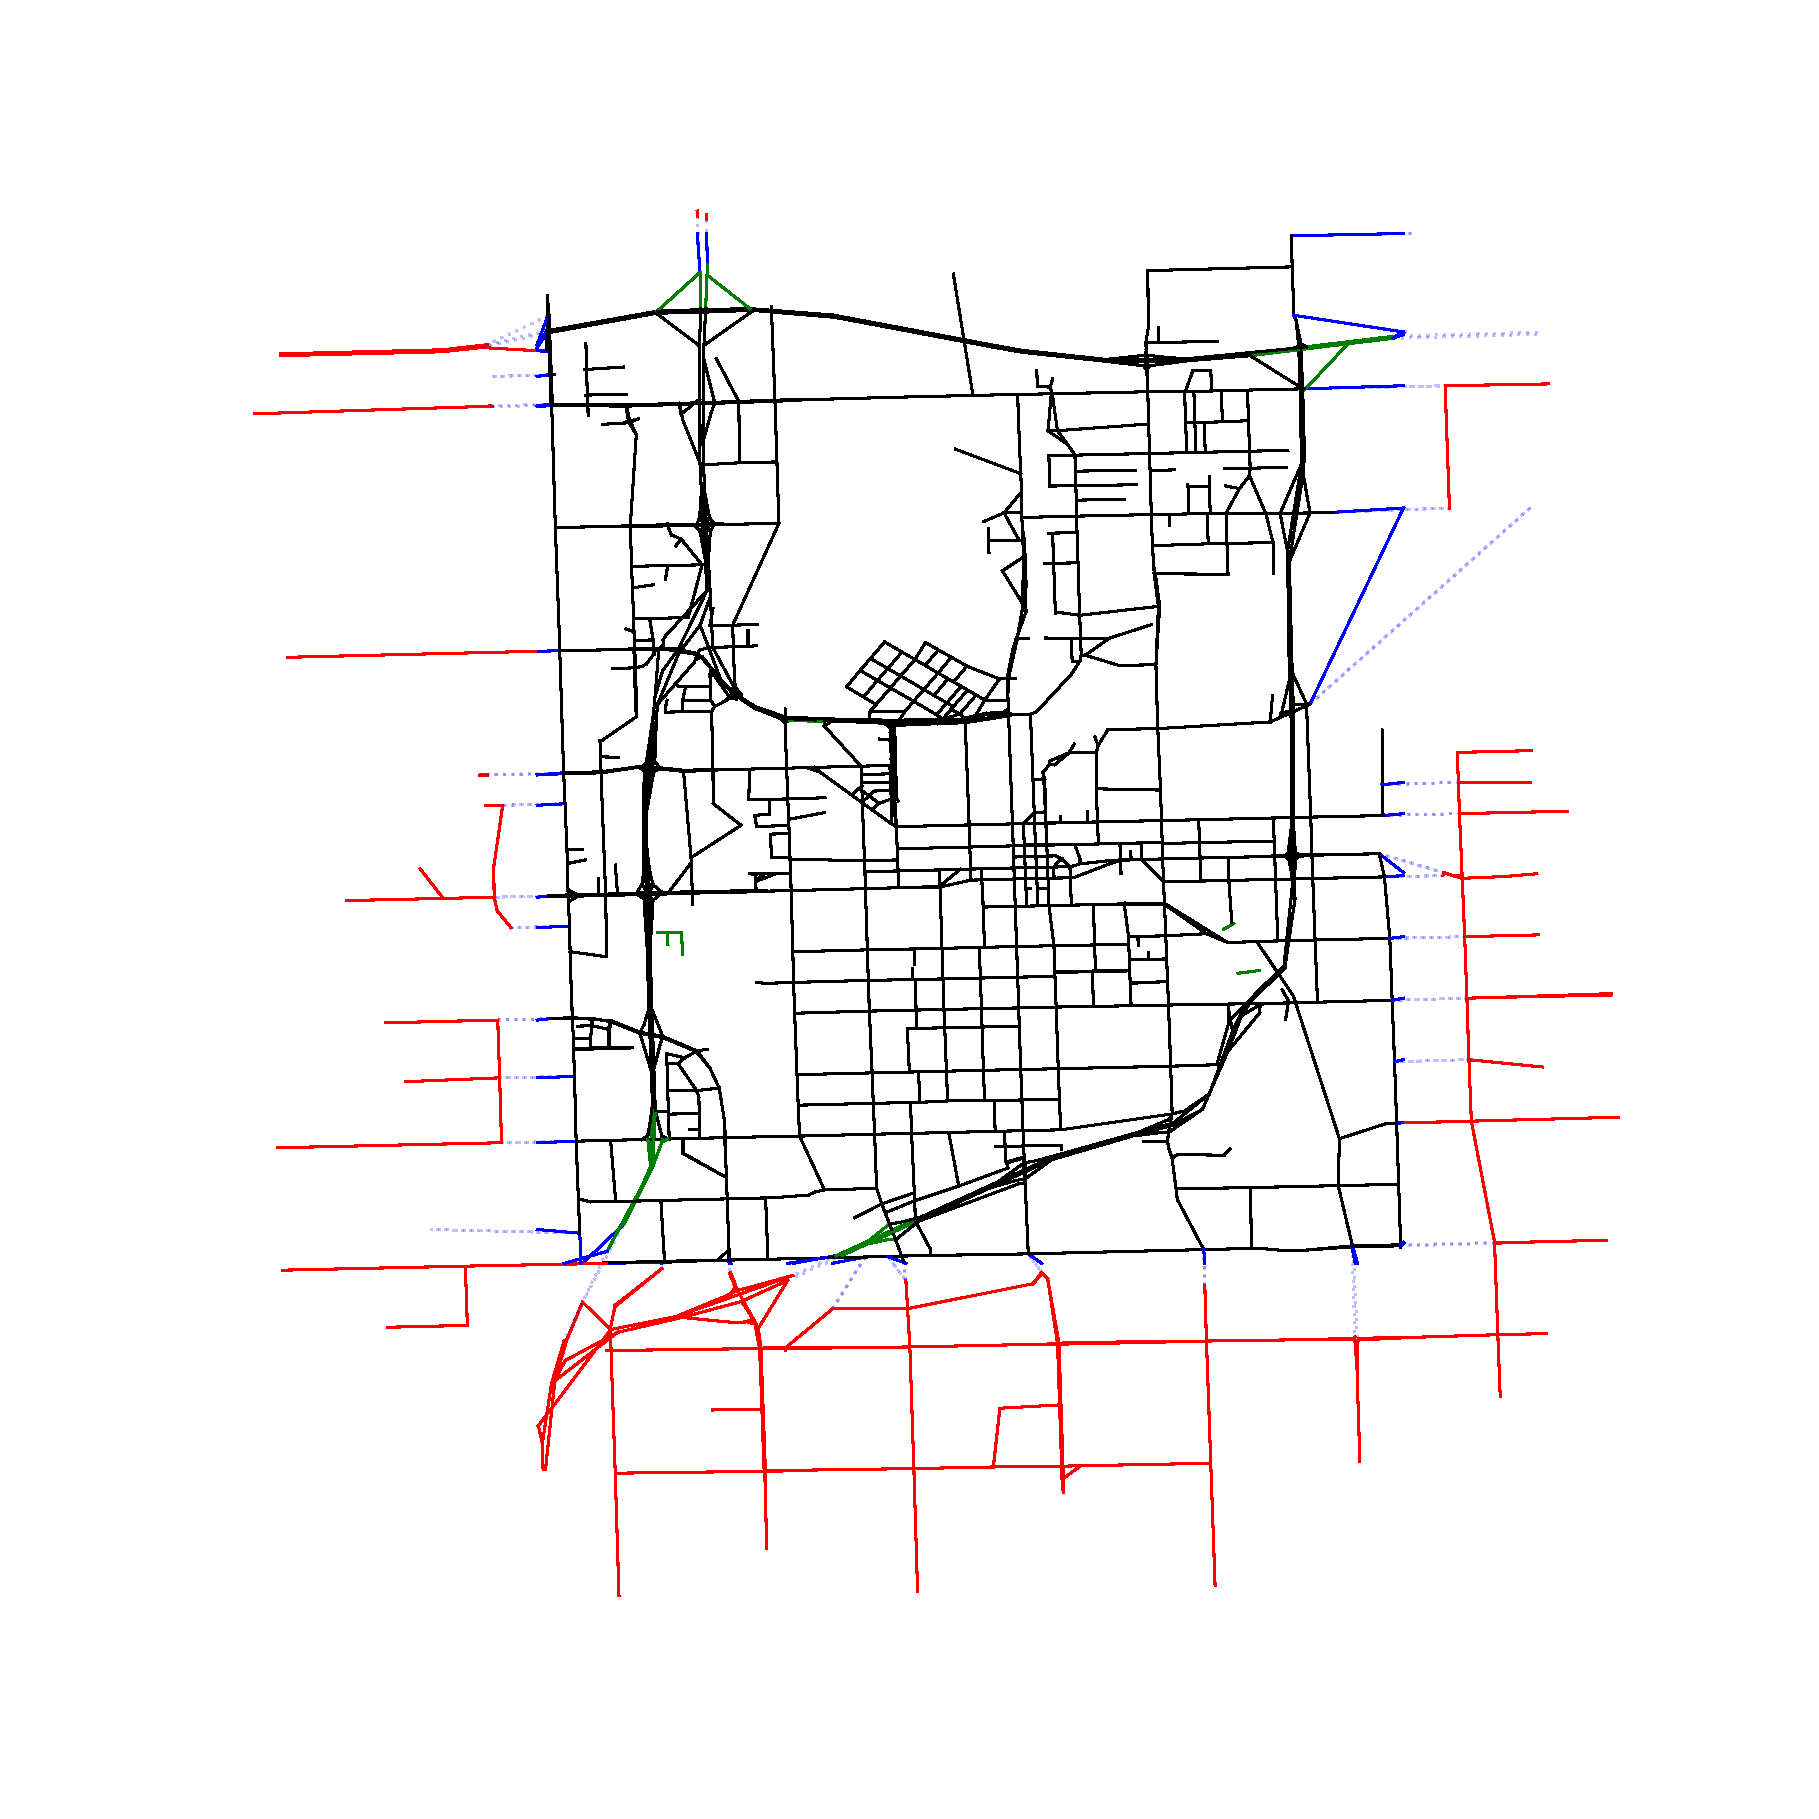
\includegraphics[width=0.6\textwidth]{figures/sioux_step2.pdf}
    \caption{Automatic network modifications: Red links have been removed while
    blue links have been shrunk to the closest border points of a bounding box
    enclosing the facilities of the scenario. Green lines have been removed either
    for being detached from the main network being sinks/sources.}
    \label{fig:sioux_step2}
\end{figure}

After that, a cleanup up the network needed to be done, partly because of artifacts
due to the filtering of road types, partly because of the removal of the external
sections. This removal was done in a couple of steps:

\begin{enumerate}
\item The lengths of all the links have been updated to the $L^2$ distance of their
respective start and end nodes in the new coordinate system.
\item The network has been searched for sources (nodes that only have outgoing links)
and sinks (nodes that only have incoming links). Those have been removed, because they
make no practical sense. This proecdure lead to 53 removed links in total.
\item One seed node has been defined, which definitely belongs to to the street
network and then by traversing the all paths from that node, it has been determined,
which streets belong to the main network. All remaining nodes and links, which have
become detached from this main network have been removed (11 nodes and 14 links).
\item Finally, the network has been searched for duplicate links with the exact
same start and end node. Only the first of those links have been kept, which lead
to the removal of 3 duplicates.
\item In Sioux-14, the links have been split such that there are no connections
longer than $500m$. This procedure has also been applied to the network at hand,
leading to 389 split links, which have been cut into a number of equal parts
with less than $500m$ length depending on their overall length.
\end{enumerate}

Regarding nodes, these procedures in total lead to an increase of nodes from
$1392$ to $1806$ and in an increase of links from $2957$ to $3335$. The links
that have been removed during the cleanup are colored in green in \cref{fig:sioux_step2}.

\subsection{Public Transport Adaptation}

The adaptation of the public transport network to the new (``Sioux-16'') scenario posed some
challenges that needed to be solved:

\begin{itemize}
\item The links of the original network did not exist anymore, obviously the
routes for the different public transport needed to be mapped to the new network.
\item The stops from the original network could not be mapped easily to the new
roads, partly because some streets in Sioux-14 were ``invented'', only approximating
connections in the finer network on a very coarse level, but also because roads
that consisted of two overimposed links for both directions were now split up into
two spatially distinct lanes (as can be seen in the upper left part of \cref{fig:pt_network}).
\end{itemize}

In order to get a rough routing for the bus lines, the main nodes of the Sioux-14
network have manually been mapped by hand to nodes in the Sioux-16 network. This
made it possible to obtain new public transport roads in terms of those guide points:
For each of the lines it has been defined, which guide points should be traversed
and in which order. Then, the Dijkstra algorithm \citep{Dijkstra} with travel time as the objective
has been used to find the shortest path from waypoint to waypoint. After fitting
those partial paths together, the whole routes in terms of the links of the Sioux-16
network have been obtained. As can be seen in the colored routes in \cref{fig:pt_network}
this made it easy to obtain routes that take into account the specific map structure
(for instance the highway on the upper left or the one-way streets, which are
traversed by the blue line in the center of the map).

The generation of bus stop facilities was a more challenging problem. Given the
location from Sioux-14, one could roughly match the stops to links along the new
routes, which worked in principle. However, using this approach, bus stops were
cluttered all along the lines. With the intention of having a rather realistic
network some conditions needed to be taken into account:

\begin{itemize}
\item The bus stops of one line should be on opposite sides of a street and not
have a large longitudial distance. While satisfiying results could obtained, for
instance in the center with the blue line, the same approaches did not work well
for the highway connectors on the left for the green line, and vice versa.
\item The bus stops of parallel lines should be at the same locations, i.e. in
the center where the green line uses the same roads as the red one, the same
locations should be chosen. This constraint usually interfered with the approaches
that took into account the first constraint (especially in the center for the
blue line).
\item Finally, some of the Sioux-14 locations where completely off the network in Sioux-16,
for instance for the red line, where one can see a bend in the diagonal connection,
which was modelled as a straight line in Sioux-14.
\end{itemize}

Given all those constraints the best approach seemed to put in manual work with
some automated help. The final approach made use of a small program, written to
manually choose the stop locations along all roads and then subsequently choose
which stop locations should belong to which line. In this step one did not take
into account the cases of two lanes, as just the general positions needed to be
known (e.g. for the blue line in the center an approximate position between the
two lines would be chosen).

In another step, the locations that had been assigned to each line have been
assigned to the respective links along the line. So for the blue one, the average
points in between would have been assigned to a link underneath for one direction,
and another stop would be created for the link above. This resulted in a final
set of stop locations.

Furthermore, some stop locations were located on one single link. This
can happen if there is a link of roughly $500m$ and the stops are for instance
located at $1m$ and $499m$ along the link. In those cases, the network needed to
be broken up at those positions. In the current scenario, this leads to the splitting
of only four links.

Finally, according to the setup of Sioux-14 the stop locations have been moved
to a position normal to the link direction, with a distance of $5m$. Additionally
a schedule with buses departing in $5min$ intervals has been created.

The final public transport network can be seen in \cref{fig:pt_network}. It features
150 stops with an average distance of $520m$ and a median of $566m$. This is a
result of not being able to put the stops as accurately in intervals of $600m$
as it is possible in Sioux-14. Moreover, the $L^2$ distance between two stops along
the routes have been used instead of a measure along the actual path. The minimum
and maximum distance between stops are $218m$ and $847m$, respectively.

All steps that have been described above have been implemented in a reusable and
parametrized way. For instance, one could choose to allow a maximum link length of
$5km$ and would still obtain a valid network at the end, probably just with a larger
number of split links during the processing of the public transport.

\begin{figure}[h]
    \centering
    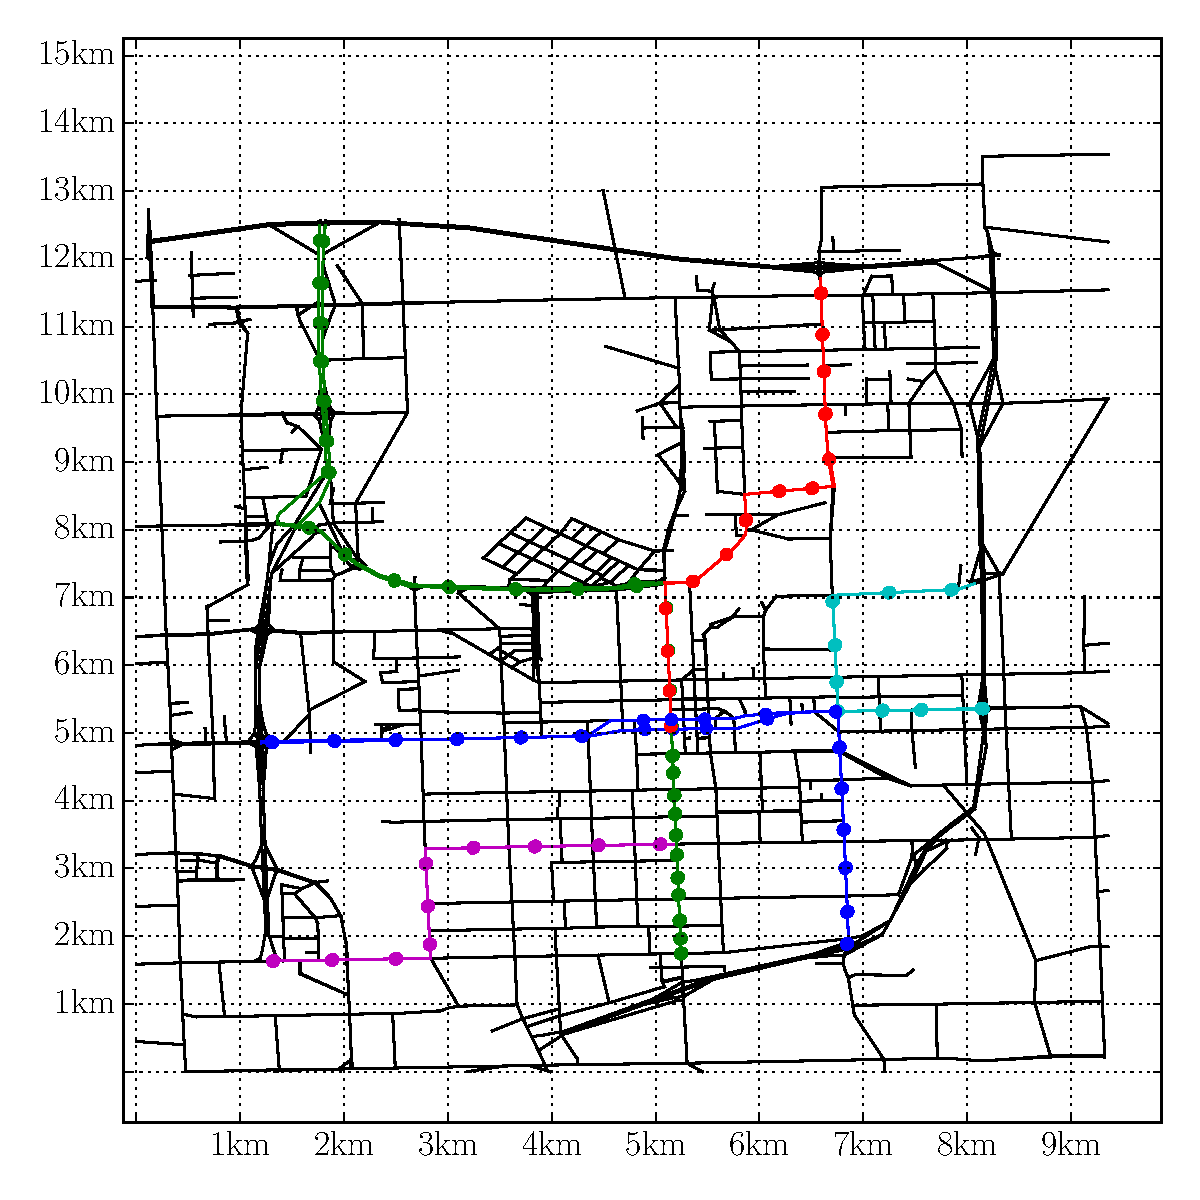
\includegraphics[width=0.9\textwidth]{figures/pt_network.pdf}
    \caption{Sioux-16 network with five public transport lines and respective stop
    facilities}
    \label{fig:pt_network}
\end{figure}

\subsection{Scenario Calibration}

The Sioux-14 network features artificially chosen link capacities, which are based
on a minimum of two and a maximum of three lanes per link, where three have only
be chosen for a fraction of highway links \citep{Chakirov2014}. While the added
minor streets in Sioux-16 should not make too much of an impact on overall
capacity, the highways and main arterials of the real network usually feature
greater capacity (for instance by providing \textit{four} lanes on the western highway).

Looking at \cref{fig:sioux_times}, it can be seen that the travel time (of cars) in
the new network is lower (red), compared to Sioux-16 (black). This effect can partly
be explained by the increased capacity, but also by the multitude of new options
to choose the most effective route for a trip through the fine-grained network. In
fact, the route choice might be the major influence when comparing with the data
from \cref{fig:sioux_speeds}. There the decrease in link speeds (relative to the freespeed) can be seen, which
is quite similar, indicating a comparable amount of congestion in the network.

Depending on how important the comparability to Sioux-14 in a specific scenario
is and what time of the day should be compared, it might be beneficial to adjust
the flow capacity of the network\footnote{In MATSim, this can be easily done
in the Mobsim configuration, e.g. \texttt{qsim.flowCapacityFactor} for QSim}:
In terms of travel times a scaling of 50\% would resemble the afternoon peak
way better than the 100\% version, while the morning peak would best be recovered
by a value in between (\cref{fig:sioux_times}). A similar situation arises for the
link speeds in \cref{fig:sioux_speeds}, where a value of 50\% is better suited for
comparing the morning peak while the 100\% scaling creates more comparable
results in the evening.

Furthermore, in terms of link speeds, it can be seen that the Sioux-16 scenario
features less congestion during the off-peak hours due to the possibility of
distributing trips all over the network.

In any case it has to be kept in mind that comparing the speed decreases is only
a rough measure of network congestion. Most importantly, the values displayed are
average values, which means that they biased towards outliers, i.e. capturing the
changes in main arterials. That is a good comparison to Sioux-14, but on the other
hand, the average is also taken over an increased number of links, of which some might rarely be
used and therefore dragging the average down.

A comparison of the scenarios in terms of average travel times, distances and more
shares can be found in \cref{tab:sioux}. What can be seen is that averaged over
the whole day, values stay roughly the same, with the biggest differences being
present in car traffic. There, especially the decrease in travel distance is
noticeable but expected, since more direct routes can be taken.
For public transport, the result of Sioux-16 is similar to Sioux-14, which is
an indicator that the network is strongly resembling the former version.

Looking at the travel time and distance for the transit walk to and from public
transport facilities, one can see that changes are quite small, which allows the
conclusion that the fine-grained network does not incline agents to switch to the
car mode on the new network. This is verified by a comparison of the mode shares,
which stay roughly constant for the scenarios. A major difference can be seen in
the mode shares of walking and public transport legs, where roughly two to three
percent of the agents in the network switch from the walking mode to public
transport.

\begin{figure}
    \centering
    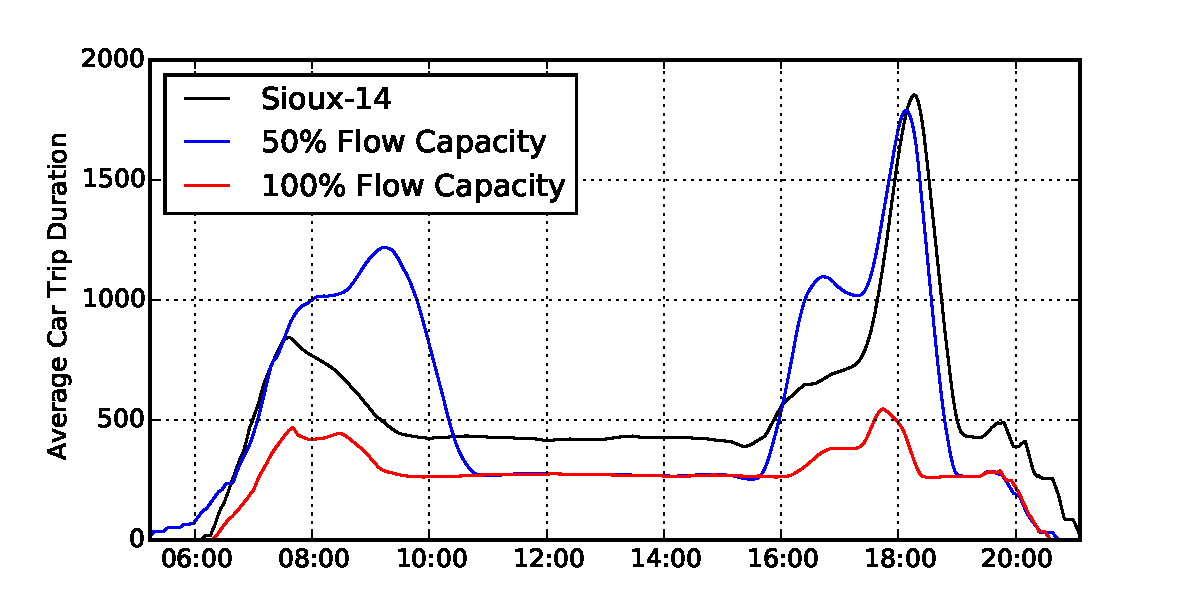
\includegraphics[width=1.0\textwidth]{figures/sioux_times.pdf}
    \caption{Comparison of the average duration of car trips by day time in Sioux-14 and Sioux-16 with 50\% and 100\% flow capacity.}
    \label{fig:sioux_times}
\end{figure}

\begin{figure}
    \centering
    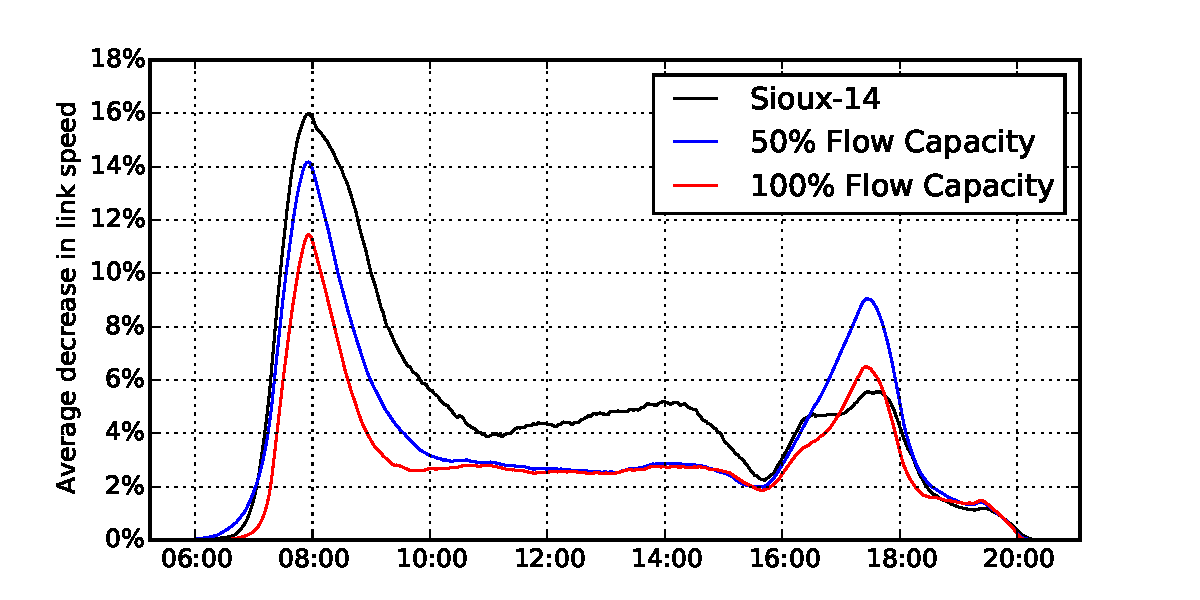
\includegraphics[width=1.0\textwidth]{figures/sioux_speeds.pdf}
    \caption{Comparison of the decrease of link speeds by day time in Sioux-14 and Sioux-16 with 50\% and 100\% flow capacity. \todo{redo this with capacity measurement instead of speed}}
    \label{fig:sioux_speeds}
\end{figure}


\begin{table}[]
\centering
\caption{Comparison of Sioux-14 and Sioux-16 in terms of travel measures. The respective
distances and travel times of the walking legs to and from public transport facilities
are included in the measures for public transport}
\label{tab:sioux}
\begin{tabular}{@{}lrrrr@{}}
\toprule
\textbf{Scenario}                  & \multicolumn{1}{c}{Sioux-14} & \multicolumn{1}{c}{Sioux-16} & \multicolumn{1}{c}{Sioux-16} & \multicolumn{1}{c}{Sioux-16} \\
Flow Capacity                      & \multicolumn{1}{c}{}         & \multicolumn{1}{c}{50\%}     & \multicolumn{1}{c}{70\%}     & \multicolumn{1}{c}{100\%}    \\ \midrule
\textbf{Travel Distances {[}km{]}} & \multicolumn{1}{l}{}         & \multicolumn{1}{l}{}         & \multicolumn{1}{l}{}         & \multicolumn{1}{l}{}         \\
Car                                & 5.30                         & 3.79                         & 3.74                         & 3.70                         \\
Walking                            & 1.31                         & 1.29                         & 1.27                         & 1.26                         \\
Public Transport                   & 3.73                         & 3.82                         & 3.86                         & 3.89                         \\
(Transit Walk)                     & 1.31                         & 0.53                         & 1.28                         & 1.28                         \\\midrule
\textbf{Travel Times {[}mm:ss{]}}  & \multicolumn{1}{l}{}         & \multicolumn{1}{l}{}         & \multicolumn{1}{l}{}         & \multicolumn{1}{l}{}         \\
Car                                & 11:56                        & 08:39                        & 06:59                        & 05:08                        \\
Walking                            & 26:16                        & 25:48                        & 25:19                        & 25:08                        \\
Public Transport                   & 32:37                        & 29:05                        & 28:32                        & 28:14                        \\
(Transit Walk)                     & 24:05                        & 21:50                        & 21:55                        & 21:59                        \\\midrule
\textbf{Mode Shares}               & \multicolumn{1}{l}{}         & \multicolumn{1}{l}{}         & \multicolumn{1}{l}{}         & \multicolumn{1}{l}{}         \\
Car                                & 63.57\%                      & 63.23\%                      & 64.84\%                      & 65.71\%                      \\
Walking                            & 9.29\%                       & 7.50\%                       & 6.80\%                       & 6.56\%                       \\
Public Transport                   & 27.14\%                      & 29.27\%                      & 28.36\%                      & 27.72\%                      \\ \bottomrule
\end{tabular}
\end{table}
